\section{Introduction and Design}

Our task is to write a sorting program in assembly.\\
\\
The sorting algorithm that was decided upon to be implemented was insertion sort. This sorting algorithm is relatively simple, making it easier to implement it in a language which can be troublesome to work with. The algorithm's time usage doesn't scale particularly well with the input size, being $O(n)$, but the ease of implementation is preferred over the running time of the algorithm.


\begin{figure}[h]
  \centering
  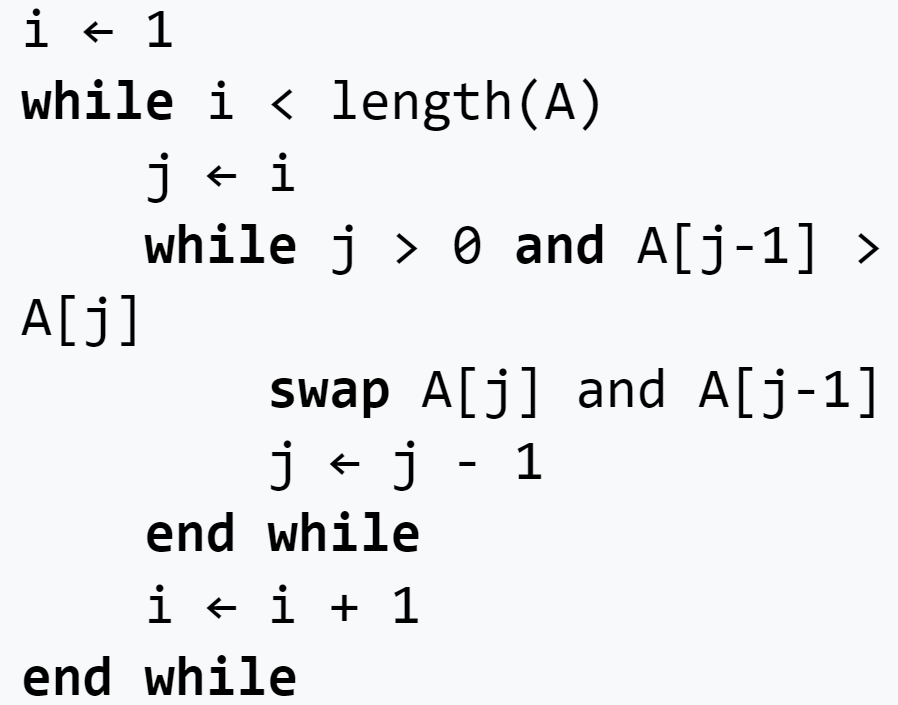
\includegraphics[width=0.40\textwidth]{insertionsort}
 \caption{psuedocode of insertionsort}
\end{figure}


%\ref{fig:originalsetup}.
%\begin{figure}[H]
%\centering
%\begin{tikzpicture}

%\draw[black] (0,0) circle (10pt) node [anchor=center] {A};
%\draw[black] (40pt,0) circle (10pt) node [anchor=center] {B};
%\draw[black,ultra thick,->] (10pt,0) -- (30pt,0);
%\draw[black,ultra thick,<-] (10pt,0) -- (30pt,0);

%\end{tikzpicture}
%\caption{Original setup}
%\label{fig:originalsetup}
%\end{figure}


%\begin{figure}[H]
%\centering
%\begin{tikzpicture}

%\draw[black] (0,0) circle (10pt) node [anchor=center] {A};
%\draw[black] (40pt,0) circle (10pt) node [anchor=center] {B};
%\draw[black] (20pt,30pt) circle (10pt) node [anchor=center] {C};

%A<->B
%\draw[black,ultra thick,->] (10pt,0) -- (30pt,0);
%\draw[black,ultra thick,<-] (10pt,0) -- (30pt,0);

%A<->C
%\draw[black,ultra thick,->] (7.07pt,7.07pt) -- (12.92pt,22.92pt);
%\draw[black,ultra thick,<-] (7.07pt,7.07pt) -- (12.92pt,22.92pt);

%B<->C
%\draw[black,ultra thick,->] (32.92pt,7.07pt) -- (27.06pt,22.92pt);
%\draw[black,ultra thick,<-] (32.92pt,7.07pt) -- (27.06pt,22.92pt);

%\end{tikzpicture}
%\caption{Three station setup}
%\label{fig:threestationsetup}
%\end{figure}
